\documentclass[11pt,english,a4paper]{report}

\usepackage[utf8]{inputenc}          % Allows UTF-8 encoded characters in the .tex-file.
\usepackage{babel,csquotes,textcomp} % Set LaTeX to structure the content following international academic standards.
\usepackage[titletoc,toc]{appendix}

\usepackage{hyperref}
\usepackage{graphicx}
\usepackage{pdfpages}
\usepackage{listings}
\usepackage{wrapfig}
\usepackage{color,colortbl}
\usepackage{lettrine}
\usepackage[font={small,it}]{caption}
\usepackage{multirow}
\usepackage{tabularx}
\usepackage{footnote}
\usepackage{enumitem}

\usepackage[
    backend=biber,
    style=numeric
]{biblatex}
\addbibresource{refs.bib}

\definecolor{mygreen}{rgb}{0,0.6,0}
\definecolor{mygray}{rgb}{0.5,0.5,0.5}
\definecolor{mymauve}{rgb}{0.58,0,0.82}

\definecolor{auxiliryc}{RGB}{70,240,161} %Green

\definecolor{ineffectivec}{RGB}{70,149,240} %purple

\definecolor{effectivec}{RGB}{115,70,240} % Blue

\lstset{ %
  basicstyle=\ttfamily\small,     
  backgroundcolor=\color{white},   % choose the background color
  breaklines=true,                 % automatic line breaking only at whitespace
  captionpos=b,                    % sets the caption-position to bottom
  commentstyle=\color{mygreen},    % comment style
  escapeinside={\%*}{*)},          % if you want to add LaTeX within your code
  keywordstyle=\color{blue},       % keyword style
  stringstyle=\color{mymauve},     % string literal style
}

\title{Report on Duqu: A collection of computer Malware}
\author{Aril Johannes Schultzen}

\begin{document}

\maketitle
\thispagestyle{empty}
\setcounter{page}{0}
%\newpage
\tableofcontents
\thispagestyle{empty}
\setcounter{page}{0}
%\newpage
\thispagestyle{empty}
\setcounter{page}{0}
%\newpage
\clearpage
\setcounter{page}{1}

\begin{abstract}
This report on Duqu (a collection of computer malware) was an assignment given in the course UNIK4740. It is mainly based on \textit{Duqu: A Stuxnet-like malware found in the wild.}\cite{DUQU_BUD} by Boldizsár Bencsáth et al (October 2011) and \textit{W32.Duqu: The precursor to the next Stuxnet}\cite{DUQU_SYMANTEC} by Symantec (November 2011). The readability of this report suffers from the level of detail it strives to achieve.
\end{abstract}
\newpage

\chapter{Introduction}
Duqu is a collection of malware discovered by The Laboratory of Cryptography and System Security (CrySyS) of the Budapest University of Technology and Economics in Hungary. They analyzed it and named it Duqu from the prefix \textasciitilde DQ that a downloaded info stealer module used to name its files. It is an interesting piece of code despite it being anything but technically astonishing. It's however interesting because of its similarities with \textit{Stuxnet} and \textit{Stuxnets} modular design and how these modules combined can be used to create a targeted threat to control systems in nuclear facilities. It is believed that the creator(s) of Duqu also created \textit{Stuxnet} or at least had access to \textit{Stuxnet's} source code. Duqu contains code that implements command and control, making it possible to control and update it as well as downloading and executing new payloads by using dummy .jpg files. Based on forensic analysis, Duqu does not self-replicate, but has in some instances been known to be instructed to replicate through the network via shares. \cite{DUQU_SYMANTEC}

\chapter{Prerequisite knowledge}
Though not a technical marvel, Duqu exploits numerous mechanisms and features in the Winodws Operating system. Some of these mechanisms will be explained in this section and should be understood before venturing further into this report.

\section{DLL}
A DLL (Dynamic Link Libraries) is Microsoft's implementation of the \textit{shared library} concept used in both Windows and the OS/2 operating system. It can contain both code and data and shares its file format with the Windows Executable file (EXE). A DLL can be used by multiple programs at the same time. The idea is that it promotes reuse of code while achieving higher memory efficiency.

\subsection{DLL Injecting and Hooking} \label{DLL_HOOKING}
A DLL injection is when a DLL is injected into the address space of an already running process. By using an already running process as opposed to making a new process to run the DLL, detection is far easier to avoid \cite{DEJAN_HOOK}. DLL Hooking or API Hooking, is a range of techniques of intercepting function calls or messages in an operating system, changing the behavior of it \cite{BREMER_HOOK}. In any case, both DLL injecting and Hooking requires administrative privileges. This means that you need complete control over the victims system before these techniques are employed. In other words, the techniques are used not to gain access, but to avoid detection. 

\subsection{Exports} \label{EXPORTS}
A DLL contains an \textit{exports table} which contains the name of every function that the DLL exposes (or exports) to other executables. A Java analogy would be the \texttt{public} modifier.

\section{Drivers}
A Driver (also known as Device driver) an abstraction layer that provides a software interface to the hardware. A driver can either be written in kernel mode or user mode. When running in kernel mode, the driver has access to every resource and all hardware, this also means that every CPU instruction can be executed and every memory address can accessed. An application written in user-mode can not directly access hardware or memory but has to use APIs instead. This isolation makes a crash in user-mode recoverable instead of catastrophic as in a kernel-mode.

\subsection{Driver Signing} \label{DRIVER_SIGN}
Digital signatures are used to demonstrate the authenticity of the producer of the driver and the integrity of the code. This can be used to protect an operating system against malicious code, for example, Microsoft Windows 7 is by default set to reject unsigned drivers.  

\section{The Windows registry}
The registry is a database used in Microsoft Windows to store settings and options. It can be considered as an alternative to the use of INI files. The use of the registry is not compulsory.

\section{RPC}
Remote Procedure Calls (RPC) is a system that allows programmers to write distributed software without worrying about the underlying network code. It is most often used to create a server/client model. \cite{MSRPC}

\chapter{Targets and Infections}
\section{Targets}
According to \textit{W32.Duqu: The precursor to the next Stuxnet}\cite{DUQU_SYMANTEC} by Symantec (November 2011), Duqu is the precursor to Stuxnet. It is believed that it was only made to gather information though with a different payload, it could do anything. Judging by infection data, it would seem as if it was made to gather intelligence from industrial infrastructure and system manufactures. This data is believed to be used for a later attack \cite{DUQU_SYMANTEC}. This makes sense if it was made by the same people as Stuxnet considering how specifically targeted it was. 

\section{Infections}
I have failed to find any detailed reports concerning specific Duqu infections. One theory explaining why, is that infected organizations are reluctant to admit that they have been victims for an attack. Publications of an infection could harm public relations and hurt customers and clients trust. However, Symantec have produced some statistics on Duqu infections and in which countries it has occurred. They claim that nine international organizations systems have been compromised:
\begin{table}[h]
        \caption{Compromised nations in victim organizations \cite{DUQU_SYMANTEC}}
        \begin{tabular}{|l|l|}
        \hline
        Organization A & France, Netherlands, Switzerland, Ukraine  \\ \hline
        Organization B & India  \\ \hline
        Organization C & Iran  \\ \hline
        Organization D & Iran  \\ \hline
        Organization E & Sudan  \\ \hline
        Organization F & Vietnam  \\ \hline
        \end{tabular}
      \end{table}

\chapter{Installation of Duqu}
The following sections covers one of the most discussed method of delivering and installing Duqu. The process is divided into two, \textit{Preparation} and the \textit{Installation}.

\section{Preparation}
Duqu was delivered to the target by using a specially crafted Microsoft Word document. According to Microsoft the Duqu malware exploits a problem in T2EMBED.DLL which is called by the TrueType font parsing engine \cite{RYAN_ZDNET}. This exploit in the Win32k TrueType font parsing engine allows arbitrary code to run in kernel mode. This arbitrary code will from now on in this report be reference to as the \textit{prep-code}. 

Once the Word document is opened and the exploit triggered, the prep-code will do a check to determine whether or not the target has been infected. This is done by checking the registry for the following value:
\begin{lstlisting}
HKEY_LOCAL_MACHINE\ SOFTWARE\Microsoft\Windows\CurrentVersion\Internet Settings\Zones\4\"CF1D" 
\end{lstlisting}
Unless the value is found, indicating that the computer is compromised, the prep-code decrypts two files from the Word document:
 \begin{enumerate}
   \item  A Driver
   \item  Main DLL
  \end{enumerate}
{\raggedright
The prep-code executes the driver which injects the \texttt{netp191.pnf} into \texttt{services.exe}. This behavior is defined by the configuration file \texttt{netp192.pnf} which is loaded and decrypted. Before the prep-code exits, it executes \texttt{netp191.pnf} and overwrite itself with zeros. 
\par}

\section{Installation}
At this point, the prep-code no longer exists in RAM, and the driver passes the execution to \texttt{netp192.pnf}. This is where things get a little tricky. During the preparation process, \texttt{netp192.pnf} was injected into \texttt{services.exe}. Now, the same DLL but launched by the driver, decrypts three files from the injected \texttt{netp192.pnf} code. These files are:
 \begin{enumerate}
   \item \texttt{netp191.pnf} (extracted from itself)
   \item A driver file, either \texttt{JMINET7.pnf} or \texttt{cmi4432.sys}. For the sake of simplicity in this report, it is assumed that the \texttt{jminet7.sys} is the driver used in this attack. \footnote{One of the differences between \texttt{jminet7.sys} and \texttt{cmi4432.sys} is that latter actually was signed (\ref{DRIVER_SIGN}) by C-Media Electronics Inc. According to the CrySys report \cite{DUQU_BUD}, the files are very similar and it is theorized that one of them provides the functionality to utilize the key logger.}
   \item The installer configuration file
  \end{enumerate}
The prep-code executes \texttt{jminet7.sys} (driver) which injects the {\raggedright \texttt{netp191.pnf} into \texttt{services.exe}. \par} This behavior is defined by the configuration file \texttt{netp192.pnf} which is loaded and decrypted. Before the prep-code exits, it executes \texttt{netp191.pnf} and overwrites itself with zeros, effectively removing its trace. 

A time frame is defined in the installer configuration file. The installer will terminate if it is executed outside this time frame. If it is not outside the time frame, the installer will pass the execution to Duqus main DLL (\texttt{netp192.pnf}) by hooking \texttt{ntdll.dll} (see \ref{DLL_HOOKING}). The main DLL has a number of exports (see \ref{app:mainexports} for all). Installation is handled by number 4 and 5. Export 4 is used to inject the main DLL into a suitable process and to pass a pointer to the three decrypted files. Export 5 drops the earlier mentioned driver used as a load point into the following directory:
\begin{lstlisting}
%System%\Drivers\ 
\end{lstlisting}
The driver's name is defined by the installation configuration file (decrypted earlier). A service is created to make sure that the load point driver is loaded every time the computer is booted. Finally, the main DLL and the installation configuration file is encrypted and named according to the definition in the installation configuration file and placed in the following directory:
\begin{lstlisting}
%Windir%\inf\ 
\end{lstlisting}

\chapter{Payload and consequences}
\section{Starting the threat}
After the installation process is completed, \texttt{jminet7.sys} is used to activate the threat at system start. It is responsible for injecting \texttt{netp192.pnf} into a specified process. The name of the process and the path to the DLL is specified in an encrypted registry value at:
\begin{lstlisting}
HKEY _ LOCAL _ MACHINE\SYSTEM\CurrentControlSet\Services\JmiNET3\FILTER
\end{lstlisting}
A key is among the fields revealed when the value is decrypted. This key is used to decrypt the main DLL stored on disk. By default the process used for injection is \texttt{services.exe} as mentioned earlier, and the DLL is stored at:
\begin{lstlisting}
%SystemDrive%\inf\netp191.pnf 
\end{lstlisting}
The driver also makes sure that the system is not booted into Safe Mode and that no debuggers are running. It then waits until the system is ready, and injects the main DLL. It also contains code that is specific for the process used for injection, making sure it uses the right memory addresses for the relevant APIs.

\section{Main DLL, Duqu's body}
The main DLL of Duqu (\texttt{netp191.pnf}) contains the payload (See \ref{app:duqu_arc}) and is responsible for loading it as well as removing the traces of Duqu after a given time. When executed, it decrypts its configuration data (\texttt{netp192.pnf}) and checks for how long it has been running. By default, Duqu has a lifetime of 30 days. This lifetime can be extended by the attackers. If it has exceeded its lifetime, it calls export 2 (see \ref{app:mainexports}) which again calls export 6. This is the routine responsible for clean-up. Duqu then might check whether or not the system is connected to the Internet by performing a DNS lookup for a domain stored in its configuration file. It then injects itself into one of the following processes:
 \begin{itemize}
   \item Explorer.exe
   \item IExplore.exe
   \item Firefox.exe
   \item Pccntmon.exe
  \end{itemize}
The main DLL also contains an RPC component. Most of the RPC exports are left unused, but the ones concerning loading of modules are used to execute the embedded resource\_302 DLL. \footnote{ According to Symantec \cite{DUQU_SYMANTEC}, the RPC component of Duqu is identical to the one used in Stuxnet}. Finally, Duqu scans for security products and injects itself into a process (see Appendix \ref{app:injection_targets}) depending on the security product found. 

\section{Payload Loader}
As previously mentioned, \texttt{resource\_302} is contained in the main DLL. Its purpose is to load and execute payloads. The payload, configuration file for command and control (more in \ref{payload}) as well as a second DLL is all compressed and contained in \texttt{resource\_302} itself. What payload to load is not configurable but hard coded in the payload file itself. The function used to load a payload does have some parameters:
 \begin{enumerate}
   \item A method that should be used to load the payload (Int)
   \item The name of the process that should be used to load the payload into RAM (String)
   \item A String (usually set to 0)
  \end{enumerate}
The methods used for loading the payload is quite complex, but the following is a simplified explanation:
  \begin{itemize}[label={}]
    \item 0: Using hook on NTDLL.DLL and call LoadLibrary sort[RANDOM].nls as a parameter. This approach is neat because it replaces functions that monitors the file sort[RANDOM].nls which doesn't even exist. When LoadLibrary is called with that parameter, it loads from a buffer in RAM rather than on a physical disk.
    \item 1: Use a template executable which is decoded from inside the loader. The template loads the DLL from a buffer and calls an export from the DLL. By populating the template with the correct memory offsets, it can find the payload in execute it. A process is chosen and overwritten. This process is created in "suspended mode"m overwritten by the template and the executed and running under a legitimate name.
    \item 2: Same as method 1, but attempts to elevate privileges before the template is executed. 
    \item 3: Same as method 2, but takes a name of running process as parameter to be overwritten.
  \end{itemize}

\section{Payload} \label{payload}
\begin{wrapfigure}{c}{0.45\textwidth} 
  \centering
  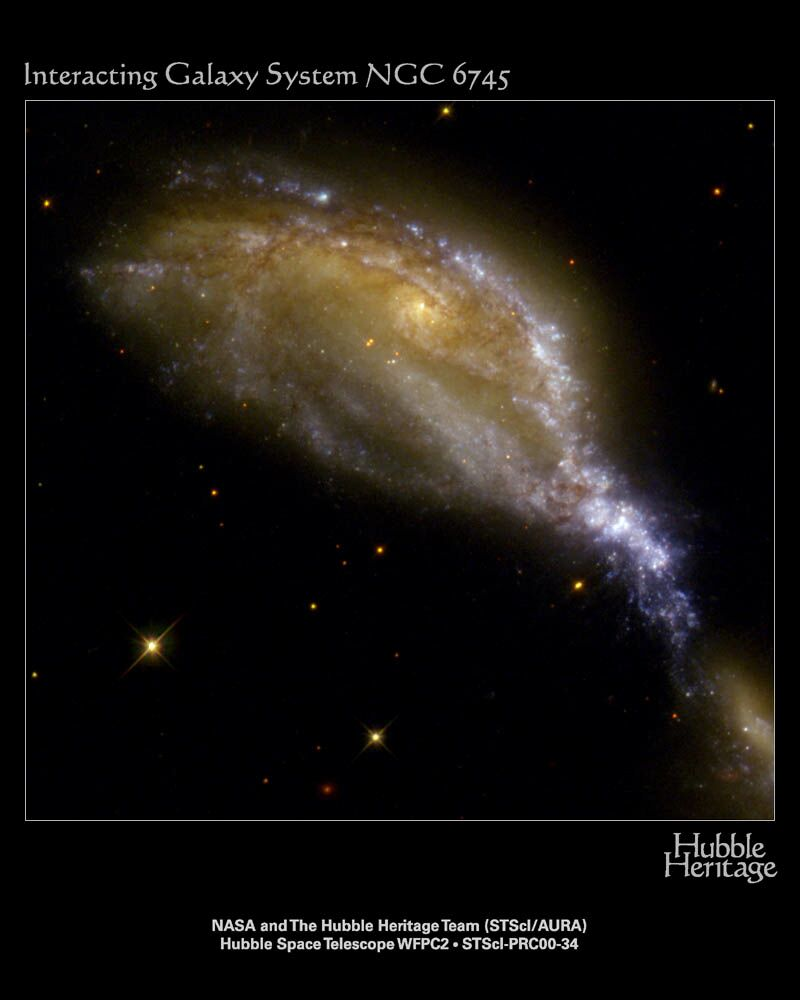
\includegraphics[width=0.40\textwidth]{hubble_duqu.jpg} 
  \caption[Hubble photo containing encrypted data]
   {Hubble photo containing encrypted data \cite{DUQU_SYMANTEC}}
   \label{hubble}
\end{wrapfigure}
Finally, the payload. It is contained in the \texttt{.zdata} section of \texttt{resource\_302} DLL. The purpose of the payload is to implement command and control functionality. This makes it possible for the attacker to download updates and new functionality to the victims system. These updates can be stored to disk or just executed directly from RAM. The command and control protocol is implemented with a custom protocol using one of the following methods:
\begin{itemize}
  \item Port 80, HTTP encapsulated
  \item Port 80, HTTP encapsulated using a proxy
  \item Port 443, HTTPS encapsulated
  \item Port 443, directly
  \item SMB Encapsulated
\end{itemize}
The configuration file will typically contain information like ports, servers and protocols to use. This way, other "clients" (or victims) can be configured to use other clients systems as proxies. Duqu also has functionality for infecting other computers on the same network, peer-to-peer. This is done over SMB (Server Message Block). Duqu can also reach a computer whose zone is considered to be secure by going through an infected computer in an insecure zone as a proxy. 

\subsection{Info stealer}
By using the command and control functionality in Duqu, attackers have been known to download and execute an "infostealer" module. The module is encrypted within an image taken by the Hubble telescope (see \ref{hubble}). When the file is executed, a DLL is extracted and an export is executed. It then steals data that it stores in the temp folder, prepending them with \textasciitilde DQ which gave Duqu its name.
The files are den compressed and XOR-encrypted. The data stolen includes information such as (but not limited to):
\begin{itemize}
  \item Running processes
  \item Names of local and shared drives
  \item Screenshots
  \item Network info
  \item Key presses
  \item Name of open windows
\end{itemize}
The info stealer module is just one example of a downloaded module. A reconnaissance module as well as an life extender module has been observed in the wild.

\chapter{Mitigation and conclusion}
\section{Mitigation steps}
Microsoft released a patch for the vulnerability in the Win32k TrueType font parsing engine (MS11-087 \cite{TT_MSB}) in  December 2011. This restricts the access to the T2EMBED.DLL effectively disabling one of Duqus known threat vectors. In general, the following actions should be done:
 \begin{enumerate}
   \item Make sure all devices connected to the system has some sort of updated security software installed.
   \item Keep all operating systems updated with the latest patches and fixes.
   \item Disable mounting of USB flash drives. 
   \item Verify the sender of emails
   \item Use extreme caution when opening Microsoft Office documents. 
  \end{enumerate}

\section{Conclusion}
The discovery of malware like Stuxnet and Duqu marks a new era in computer security. It shows how code, written for computers can affect something physical like Stuxnets influence on the centrifuge structure at the Natanz nuclear enrichment lab in Iran. It also shows how much resources someone is willing to put into malware development. Duqu is believed to be used to gather information, meaning that it's purpose is only a part of a bigger plan. It's a sober reminder that a digital certificate authority can be bypassed and that its architecture probably needs some rethinking. 

\begin{appendices}
  \chapter{NETP191.PNF Exports} \label{app:mainexports}
    \begin{table}[h]
        \caption{Table of NETP191.PNF exports \cite{DUQU_SYMANTEC}}
        \begin{tabular}{|l|l|}
        \hline
        \cellcolor[gray]{0.8} Export & \cellcolor[gray]{0.8} Function \\ \hline
        1 & Data initializer \\ \hline
        2 & Run export 6  \\ \hline
        3 & Get version info from configuration data \\ \hline
        4 & Inject self into process, run export 5 (32-bit only) \\ \hline
        5 & \begin{tabular}[c]{@{}l@{}}Setup, depends on install status.\\ Before install: Drop provided load point driver and create service.\\ After install: Load resource\_302\end{tabular} \\ \hline
        6 & Routine for cleanup \\ \hline
        7 & Start RPC \\ \hline
        8 & Identical to export 1, but uses a delay timer. \\ \hline
        \end{tabular}
      \end{table}

\chapter{Security products and injection targets} \label{app:injection_targets}
    \begin{table}[h]
        \caption{Table of processes scanned for by Duqu \cite{DUQU_SYMANTEC}}
        \begin{tabular}{|l|l|}
        \hline
        \cellcolor[gray]{0.8} Product & \cellcolor[gray]{0.8} Injection Target \\ \hline
        Kaspersky Antivirus (V.1 - 7) & lsass.exe \\ \hline
        Kaspersky Antivirus (V.8 - 11) & Kaspersky proc \\ \hline
        McAfee & Winlogon.exe \\ \hline
        AntiVir & lsass.exe \\ \hline
        Bitdefender & lsass.exe \\ \hline
        Etrust (5 and 6) & does not inject \\ \hline
        Etrust (other) & lsass.exe \\ \hline
        Symantec & lsass.exe \\ \hline
        ESET NOD32 & lsass.exe \\ \hline
        Trend & Trend proc \\ \hline
        Rising & Rising proc \\ \hline
        \end{tabular}
      \end{table}

  \chapter{Duqu architecture} \label{app:duqu_arc}
    \begin{figure}[hb]
      \centering
      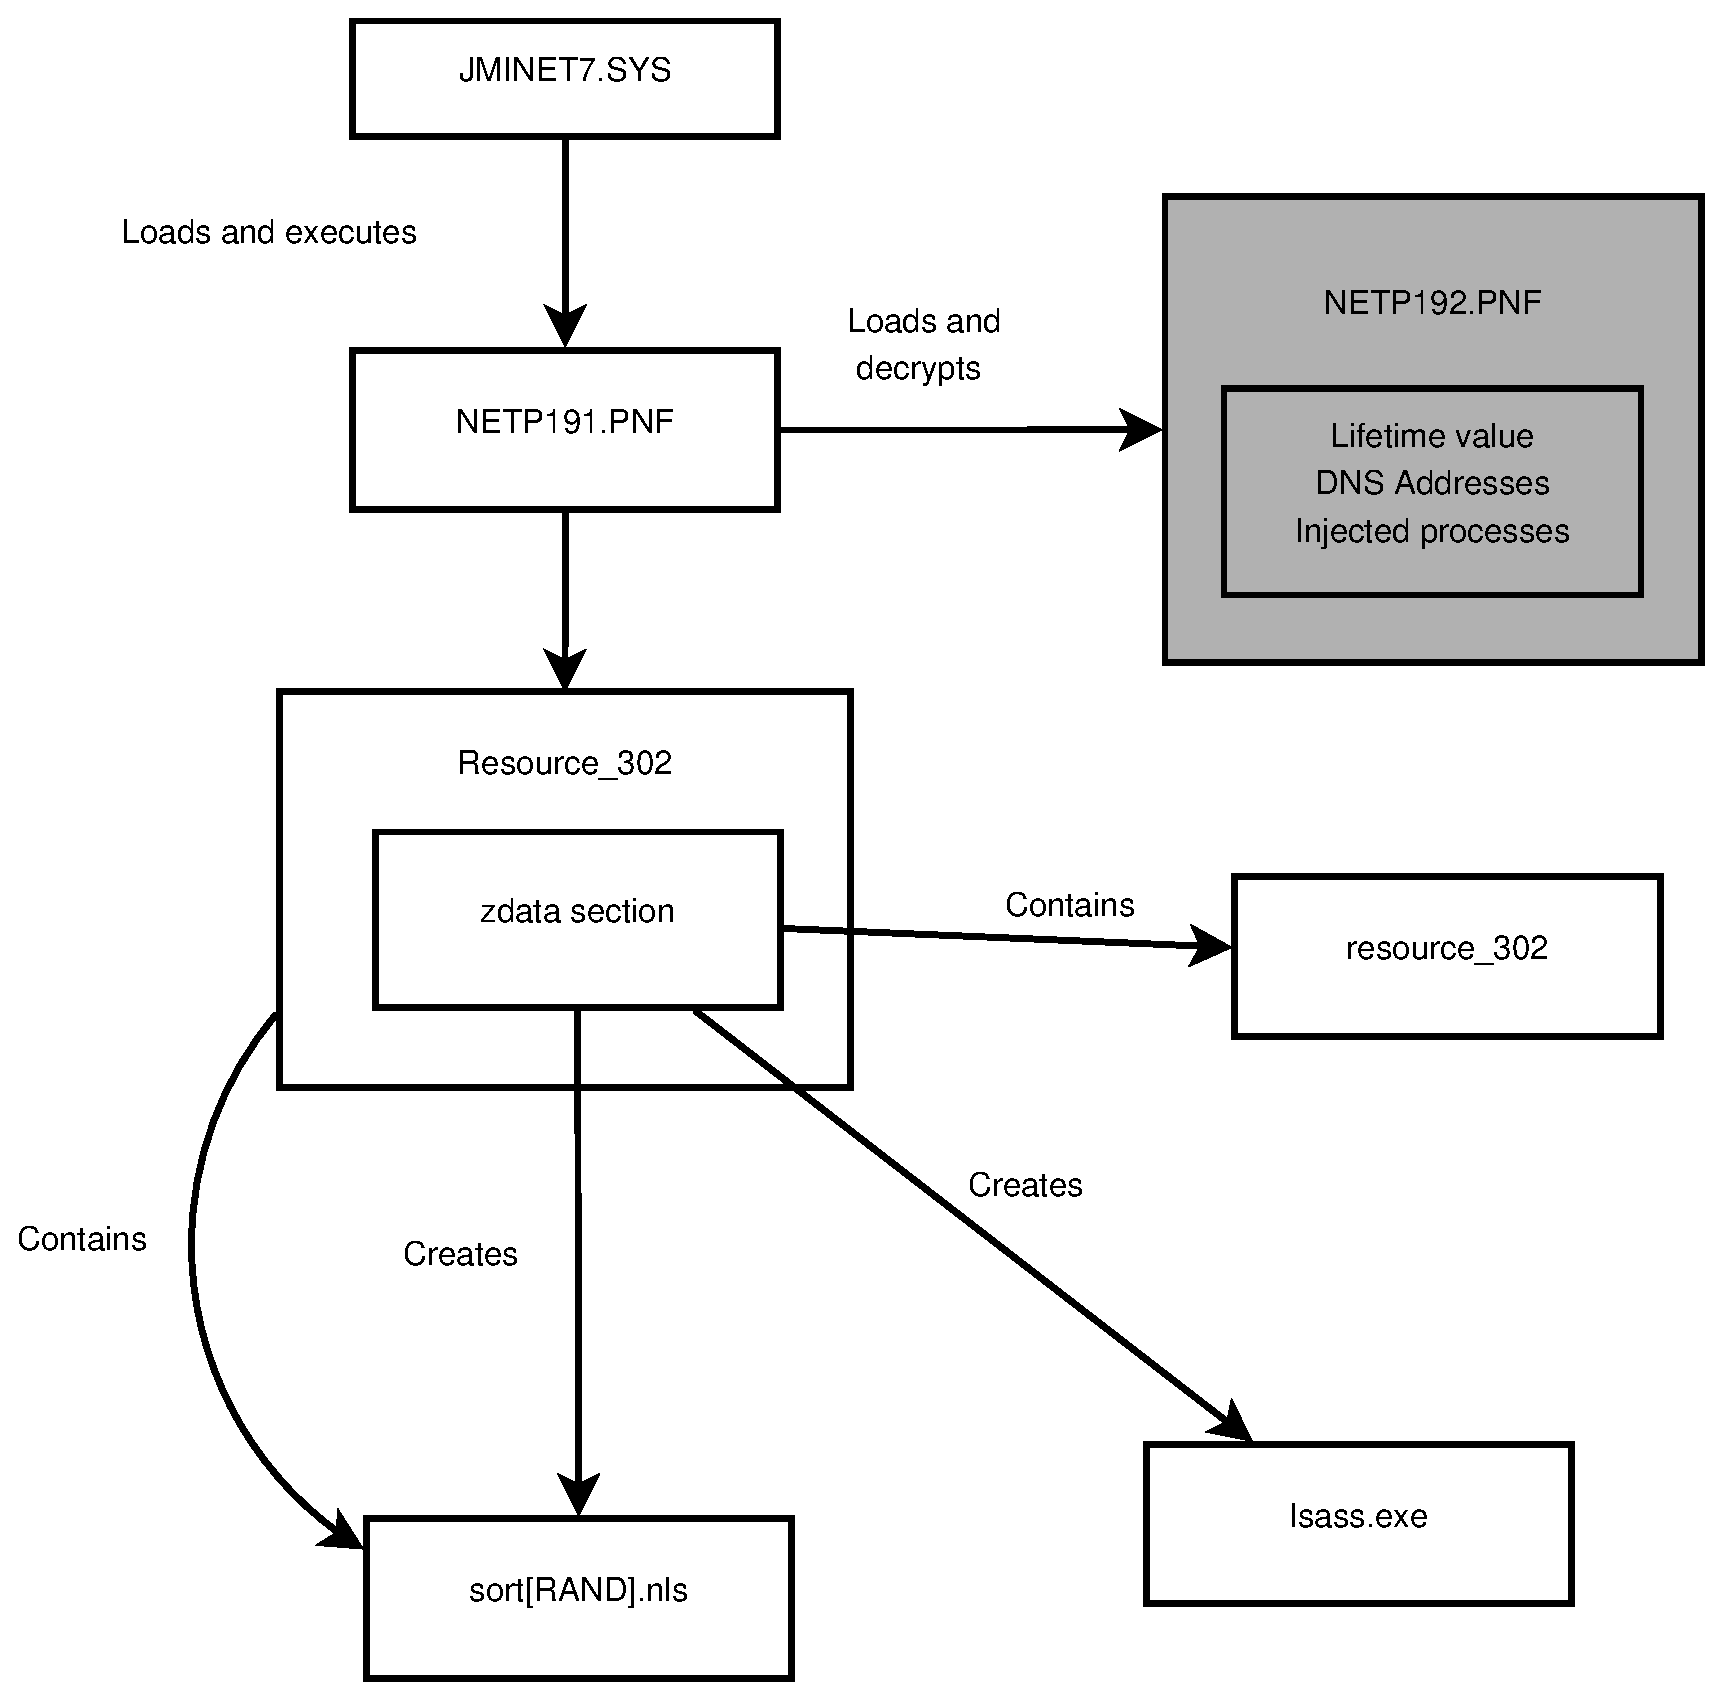
\includegraphics[width=0.90\textwidth]{duqu_arc.eps}
      \caption[File system anatomy] {Diagram showing the architecture of Duqu once installed. \cite{DUQU_SYMANTEC}} 
    \end{figure}

\end{appendices}

\newpage
\printbibliography[title={Complete Bibliography},heading=bibintoc]
\end{document}                     